\documentclass[10pt]{article}
\usepackage{longtable}
\usepackage{float}
\usepackage{wrapfig}
\usepackage{rotating}
\usepackage[normalem]{ulem}
\usepackage{amsmath}
\usepackage{textcomp}
\usepackage{marvosym}
\usepackage{wasysym}
\usepackage{amssymb}
\usepackage{hyperref}
\usepackage{color,soul} % for highlighting
\usepackage{graphicx}
\graphicspath{{/Users/benjaminbass/seacloud/class/earthMaterials/picBank/}}

\usepackage{frame,color}
\usepackage{framed}
\usepackage{minibox}

% \usepackage[T1]{fontenc}
% \usepackage{tilting} %bring title up
% \setlength{\droptitle}{-10cm}

\usepackage[version=3]{mhchem}
% How to Use MChem
% \ce{SO4^2-}
% \ce{^{227}_{90}Th+}
% \ce{A\bond{-}B\bond{=}C\bond{#}D}
% \ce{CO2 + C -> 2CO}
% \ce{SO4^2- + Ba^2+ -> BaSO4 v}


\author{Benjamin Bass}
\date{2 March 2016}
\title{\vspace{-2.0cm}Muscovite} %bring title up temporary Fix

\begin{document}

\maketitle

% \framebox{Use frameboxes until figure out alignmen}

\begin{center}
  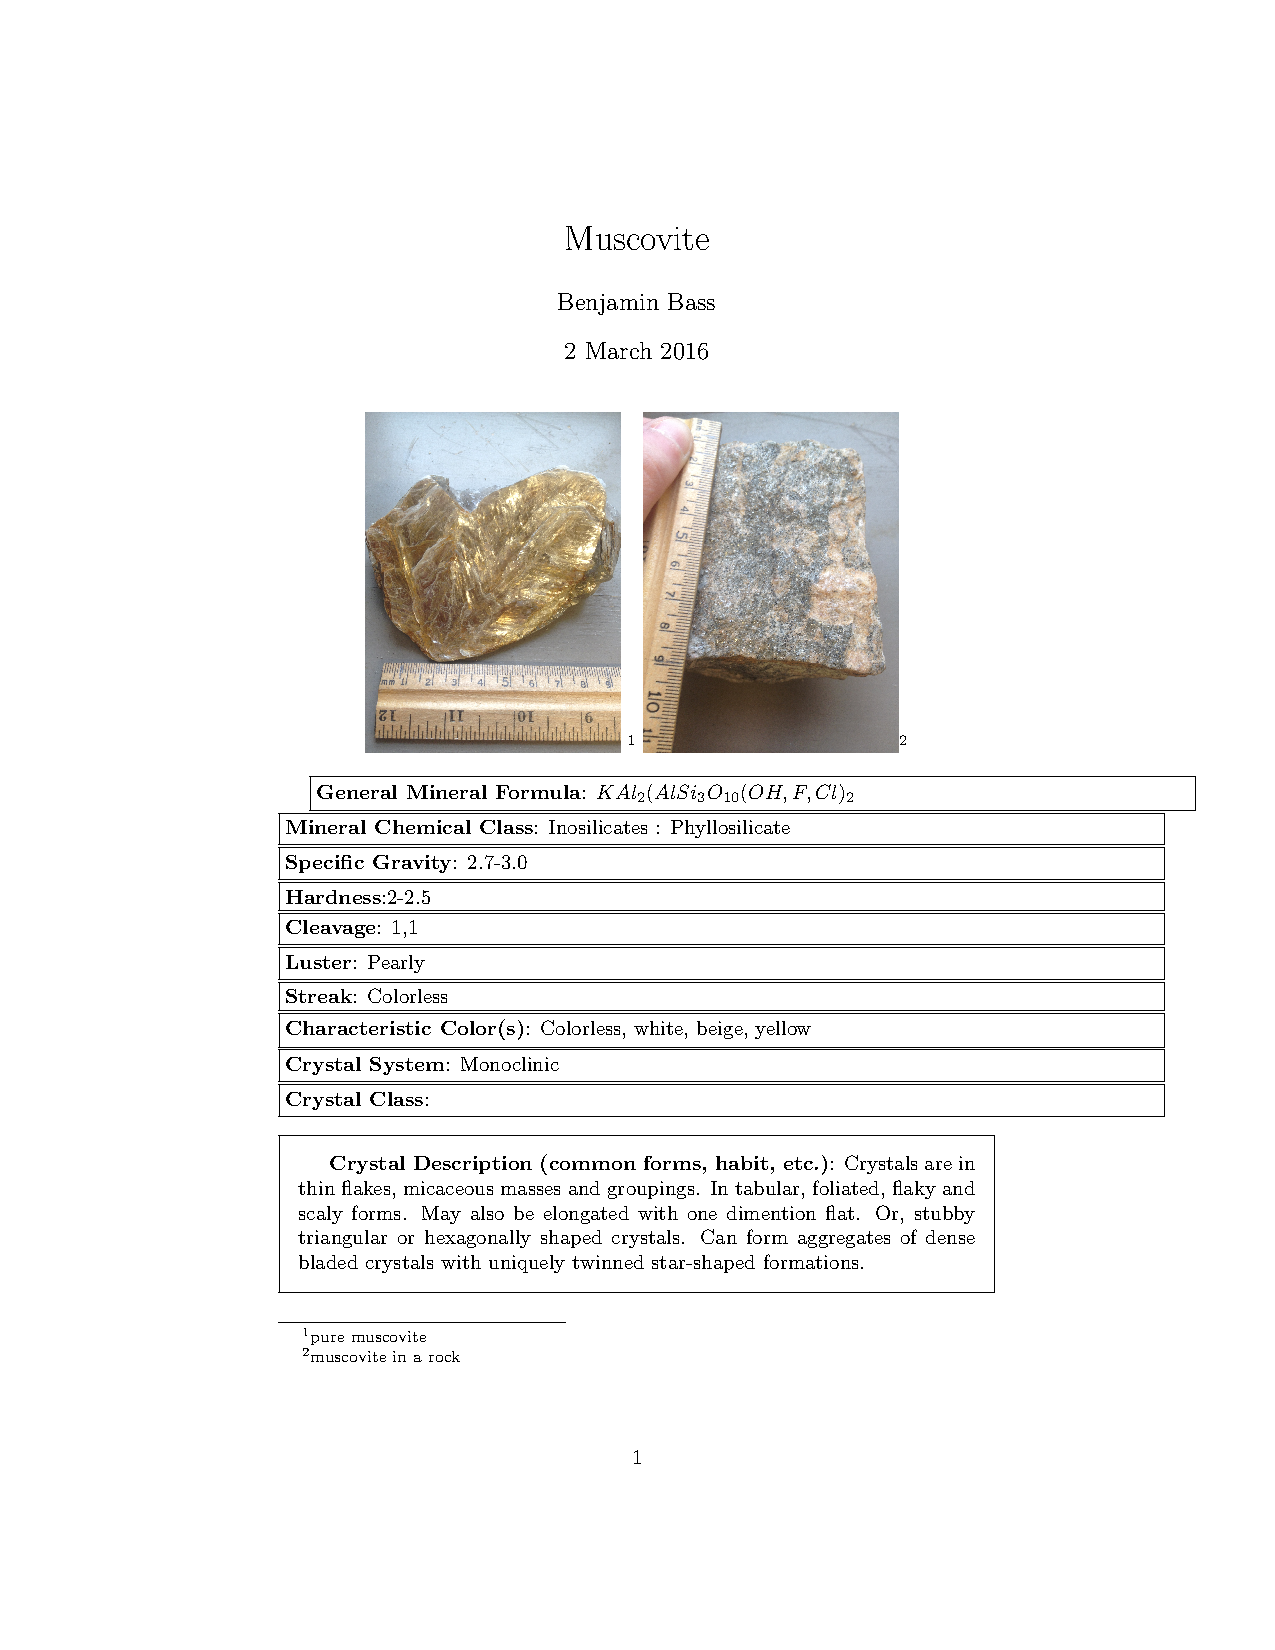
\includegraphics[scale=.05]{muscovite}\footnote{Pure muscovite: Perfect cleavage. Colorless}
  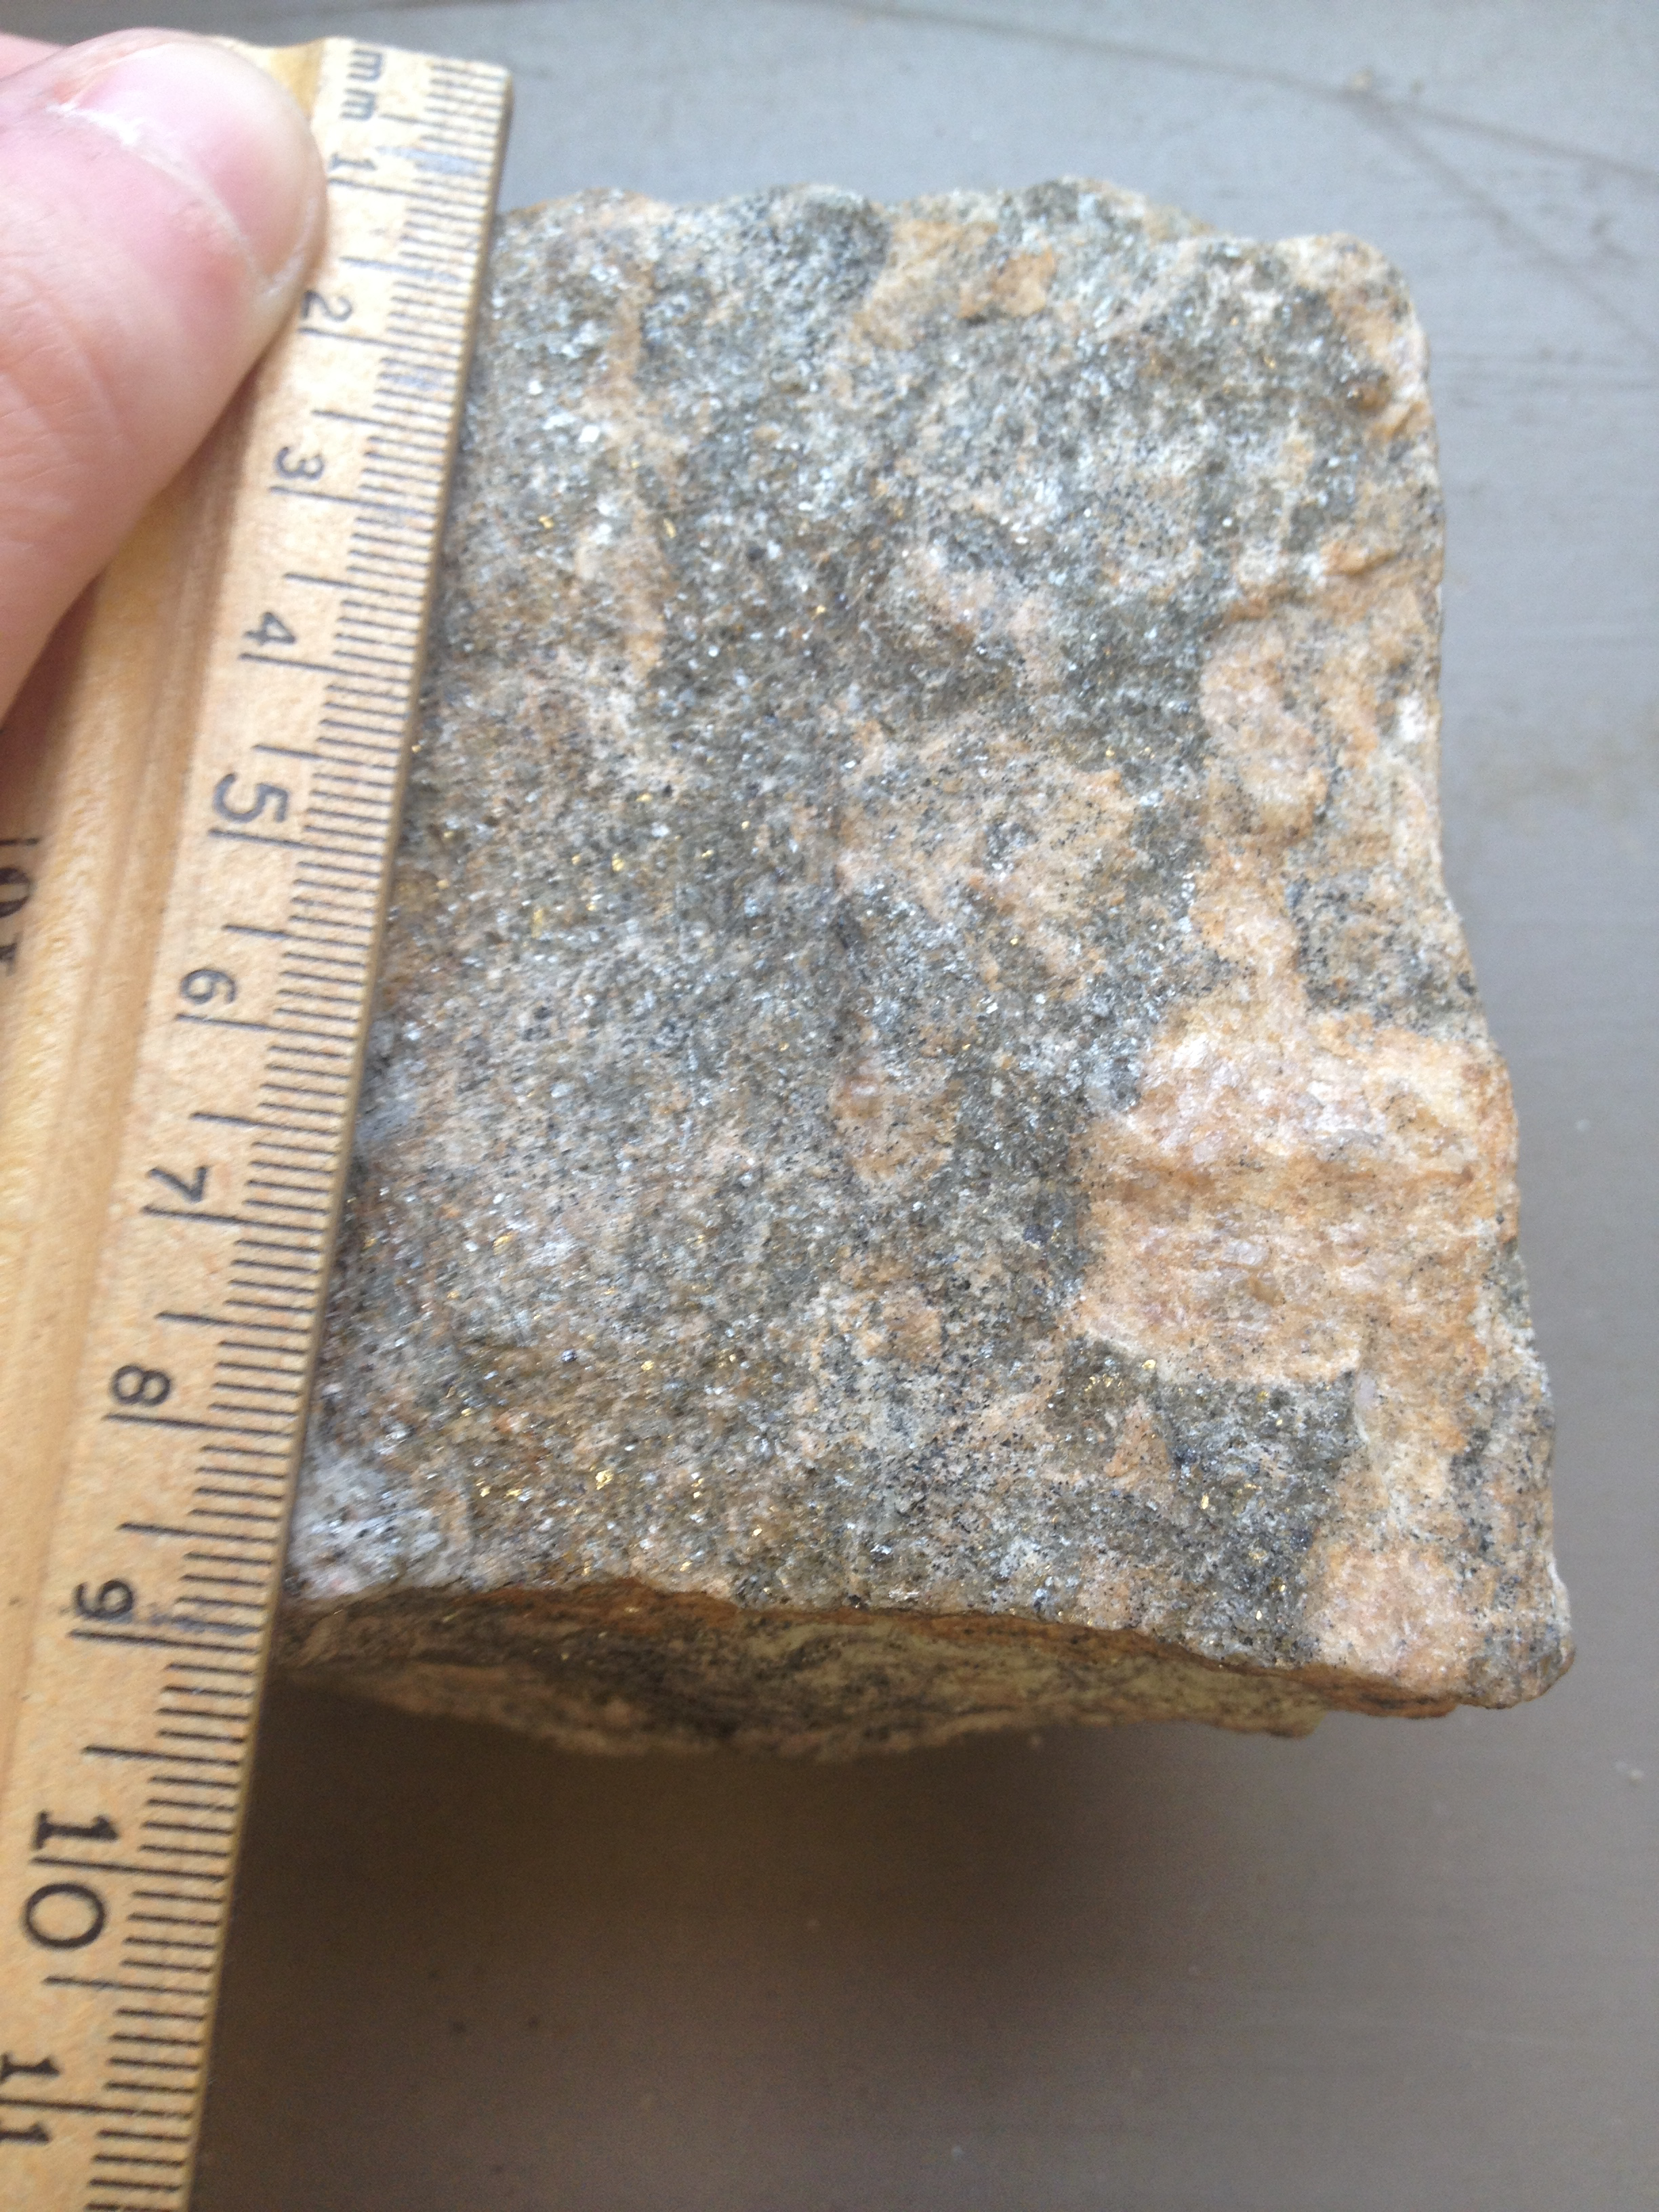
\includegraphics[scale=.05]{muscovite_inarock}\footnote{Muscovite in a rock: present in all pelitic metamorphic rocks and s-types granites.}
\end{center}



\framebox[15cm][l]{\textbf{General Mineral Formula}: $KAl_{2}(AlSi_{3}O_{10}(OH, F, Cl)_{2}$ }\
\framebox[15cm][l]{\textbf{Mineral Chemical Class}: Phyllosilicate }\
\framebox[15cm][l]{\textbf{Specific Gravity}: 2.7-3.0 }\
\framebox[15cm][l]{\textbf{Hardness}:2-2.5 }\
\framebox[15cm][l]{\textbf{Cleavage}: \hl{1,1 Perfect Cleavage. Also flexible and elastic pieces.}}\
\framebox[15cm][l]{\textbf{Luster}: Pearly  }\
\framebox[15cm][l]{\textbf{Streak}: Colorless }\
\framebox[15cm][l]{\textbf{Characteristic Color(s)}: \hl{Colorless, white, beige, yellow} }\
\framebox[15cm][l]{\textbf{Crystal System}: Monoclinic }\
\framebox[15cm][l]{\textbf{Crystal Class}: 2/\it{m} }\

\begin{framed}
  \textbf{Crystal Description (common forms, habit, etc.)}: \hl{Crystals are in thin flakes, micaceous masses and groupings. In tabular, foliated, flaky and scaly forms. May also be elongated with one dimention flat. Or, stubby triangular or hexagonally shaped crystals. Can form aggregates of dense bladed crystals with uniquely twinned star-shaped formations.}
\end{framed}

\begin{framed}
  \textbf{Environment (where you find the material}: Very common rock forming mineral. Found in granite pegmatites and contact metamorphic rocks and metamorphic schists or hydrothermal veins.
\end{framed}

\begin{framed}
  \textbf{Common Mineral Associations (in samples, also consult text, notes}: Albite, quartz, mirocline
\end{framed}

\begin{framed}
  \textbf{Scientific Usage/Significance}: Heavily used in electic circuits. Treatment for colitis and digestive track problems.
\end{framed}

\begin{framed}
  \textbf{Industrial or Social Use/Significance}: Insulator for various electircal products and semiconductors. Also used to produce automotive tires and cosmetics. Large sheets once used for oven windows.
\end{framed}

\begin{framed}
  \textbf{Environmental Significance}: A constituent of driling mud used in the drilling for oil and gas.
\end{framed}

% Possible other Solutions
% \framebox(300,20){\minibox{\textbf{R-Sq}:For example}}

\end{document}
%%% Local Variables:
%%% mode: latex
%%% TeX-master: t
%%% End:
